\documentclass[prd,preprintnumbers,floatfix,
nofootinbib,superscriptaddress]{revtex4}

%------------------

\usepackage{float}
\usepackage{nicefrac}
\usepackage{mathtools}
\usepackage{amsfonts}
\usepackage{amssymb}
\usepackage{amsmath}
\usepackage{graphicx}
\usepackage{subfigure}
\usepackage{array}
\usepackage{dcolumn}
\usepackage{bm}
\usepackage{esint}
\usepackage{xcolor}
\usepackage{longtable} % long tables
\usepackage{hyperref}
\usepackage{verbatim}
\usepackage{epsfig}
\usepackage{slashed}
\usepackage{color}


\newcommand{\diff}{\mathrm{d}}
\newcommand{\ket}[1]{\ensuremath{\left|#1\right\rangle}}
\newcommand{\bra}[1]{\ensuremath{\left\langle #1\right|}}
\newcommand{\braket}[2]{\ensuremath{\left\langle #1|#2\right\rangle}}
\newcommand{\TS}{\mathrm{TS}}
\newcommand{\LLH}{\mathrm{LLH}}
\newcommand{\M}{\mathcal{M}}
%
\newcommand{\I}{\ensuremath{I}}
\newcommand{\II}{\ensuremath{{I\!I}}}
\newcommand{\III}{\ensuremath{{I\!I\!I}}}
\newcommand{\IV}{\ensuremath{{I\!V}}}

\begin{document}
\title{Parity and signature test for the vector-vector system (revisited)}

%%%%%%%%%%
\author{Mikhail Mikhasenko}
\email[e-mail: ]{mikhail.mikhasenko@cern.ch}
\affiliation{CERN-EP, CH-1211, Geneva, Switzerland}
%%%%%%%%%%

%%%%%%%%%%
\date{\today}
%%%%%%%%%%

%%%%%%%%%%
\begin{abstract}
  We present a construction of the reaction amplitude
  for inclusive production of the resonance decaying to a pair of identical vectors, as $J/\psi J/\psi$, $\phi\phi$, $Z^0 Z^0$.
  The method provides possibility to determine the spin and parity of the resonance in the model-independent way.
  The test of the quantum-number hypotheses is demonstrated on the Standard Model decay of the Higgs particle to four leptons.
\end{abstract}
%%%%%%%%%%

\nopagebreak
\maketitle

\definecolor{cola}{rgb}{0.9,0.62,0.0}
\definecolor{colb}{rgb}{0.337, 0.706, 0.914 }
\definecolor{colc}{rgb}{0.0, 0.62, 0.451}
%
\section{Introduction}

Formation of the hadronic matter is one of a few ununderstood parts of Quantum Chromodynamics (QCD) leaving a little black spot in the Standard Model.
Despite the fact that QCD is the fundamental theory of strong interaction,
the theory degrees of freedom change at the low energy where hadronic phenomena emerges.
Whilst the constituent quark model successfully describes the majority of the observed hadronic states, not all.
Over the last decade we have witnessed overwhelming evidence of unexpected phenomena beyond the quark model that
includes the observation of $XYZ$ states in the charminium spectrum~\cite{Godfrey:2008nc}, the pentaquark states~\cite{Aaij:2015tga,Aaij:2019vzc},
as well as the resonance-like phenomena of the hadron rescattering singularizes~\cite{Alexeev:2020lvq}.
The spin-parity of the observed exotica is a critical part of the formation puzzle, and moreover, in most of the cases it can be determined experimentally.
Nevertheless, the separation of the spin hypothesis is often rather cumbersome and requires case-by-case treatment.
In the paper we revisit the problem of the spin-parity assignment for the system two identical vectors with their possible further decay.

We anticipate three applications of the presented framework.
First, the fresh observation of the threshold enhancement in the $J/\psi J/\psi$ spectrum~\cite{Aaij:2020xyz}
that might lead to a new milestone in the understanding of the hadron formation through the mechanism for binding four charm quarks~\cite{Liu:2019zoy}.
Second, the $\phi\phi$ pairs produced in central exclusive reactions hint a resonance signal, that is a candidate for a tensor glueball~\cite{Lebiedowicz:2019jru}.
The proposed approach sets the ground for the complete partial wave analysis of the high statistics $pp\to pp\,K^+K^-K^+K^-$ that
should be possible with the modern LHC data.
Thirdly, one find the same vector-vector signature in the Standard Model (SM) decay of the Higgs boson, $H\to Z^0Z^0$.
To conclude in favor of $0^+$ hypothesis for the spin-parity of the Higgs boson
several phenomenological models were compared on the combined dataset of several decay channels~\cite{Aad:2013xqa,CMS:2018mmw}.
In contrast, we discuss the anatomy of the assumption-free approach.

The two key constraints that determine the properties of the decay are the parity conservation and the permutation symmetry.
One consequence of these constraints is known as the Landau-Yang theorem~\cite{Yang:1950rg,Landau:1948kw}.
The theorem states that a massive boson with $J^P = 1^\pm$ cannot decay into two on-shell photons.
The statement follows naturally from the general equations we provide. Moreover, the extension of the selection rule to all the natural quantum numbers with odd spin is easily obtained.
A parity-signature test of a signal in $\phi\phi$ system have been discussed in the past by several authors~\cite{Trueman:1978kh,Chang:1978jb,Collins:1977iv,Trueman:1978kh,Trueman:1978kh}.
We derive the results consistent with the previous works using the modern conventions on the state vectors and rotation matrices.
Also, we suggest exploring the spin-parity hypothesis using the full power of the multidimensional test statistics.

The paper is organized as follows. The reaction amplitude is presented in Sec.~\ref{sec:reaction.amplitude}.
In Sec.~\ref{sec:symmetries} we discuss the symmetry constraints.
We describe the test-statistics discriminator in Sec.~\ref{sec:test.statistics}.
The method is demonstrated on the SM Higgs decay in Sec.~\ref{sec:higgs}.

%                                      _|  _|    _|                      _|
%    _|_|_|  _|_|_|  _|_|    _|_|_|    _|      _|_|_|_|  _|    _|    _|_|_|    _|_|
%  _|    _|  _|    _|    _|  _|    _|  _|  _|    _|      _|    _|  _|    _|  _|_|_|_|
%  _|    _|  _|    _|    _|  _|    _|  _|  _|    _|      _|    _|  _|    _|  _|
%    _|_|_|  _|    _|    _|  _|_|_|    _|  _|      _|_|    _|_|_|    _|_|_|    _|_|_|
%                            _|
%                            _|

\section{Angular amplitude} \label{sec:reaction.amplitude}
We focus on an inclusive production process $p p'\to X + \dots$, where $X$ is a resonance decaying to two vector mesons.
Despite the vectors are identical, it is convenient to distinguish them in the reaction amplitude calling them $V_1$ and $V_2$.
In that way, we can make sure that the amplitude is symmetric on the permutation of indices $1$ and $2$.

A negligibly small polarization is measured in the prompt production of charmonium~\cite{Aaij:2013nlm,Chatrchyan:2012woa,CDF:2011ag, Aaij:2013oxa,Sirunyan:2018bfd}.
In opposite, for the peripheral processes, e.g. central exclusive production (CEP) a significant polarization is expected~\cite{Pasechnik:2010pq}.
Therefore, we consider a general case of arbitrary polarization. For numerical tests however we restrict ourselves to the unpolarized case.

The production frame is set up in the rest frame of $X$ as a plane that contains three-vectors of the
production reaction, i.e. $\vec p$, and $\vec p'$. The normal to the plane gives $y$ axis (precisely $\vec p\,'\times \vec p$) as shown in Fig.~\ref{fig:production}.
We use the Gottfried-Jackson (GJ) frame for defining in the $x$ and $z$ axis in the production plane~\cite{Gottfried:1964nx}.
We note, however, that the choice of $x$ and $z$ axes is not unique, two other two common definition of the production frame are the helicity (HX) frame
defined by the direction of motion of $X$ itself in the lab frame, and the Collins-Soper (CS) frame where $z$ is defined by bisection of the angle between $\vec p$ and $\vec p\,'$~\cite{Faccioli:2010kd}.
\begin{figure}
  \includegraphics[width=0.6\textwidth]{../plots/production_GJ.pdf}
  \caption{Schematic view of production kinematics of $X$ state at the $pp$ collider.
  The Gottfried-Jackson frame is used for describing production kinematics.
  It is defined in the rest frame of $X$ by the vectors of the beam particles:
  $\vec z = \vec p / |\vec p|$, $\vec y = \vec p' \times \vec p / |\vec p' \times \vec p|$, $\vec x = \vec y \times \vec z$.
  The spherical angles $(\theta,\phi)$ are the angles of one of two decay vectors in the GJ frame.
  The black arrows shows three dimensional vectors of particles.
  The three-momenta of the produced vectors are $\vec p_{V_1}$ and $\vec p_{V_2}$.
  }
  \label{fig:production}
\end{figure}

The full kinematics of the decay is described by 6 angles: a pair of sperical angles $(\theta,\phi)$ of the momentum of $V_1$ in the GJ frame, and two pairs of the spherical angles $(\theta_i,\phi_i)$, $i=1,2$
for decay of the vectors in their own helicity frames.
We note that the angles $\phi_i$ can also be defined in the $X$ rest frame as shown in Fig.~\ref{fig:decay}
since they do not effected by the boosts.

The spin of the decay particle defines rotational properties of the system of the decay products~\cite{Mikhasenko:2019rjf}.
Every configuration of the three-momenta of the final state particles in the $X$ rest frame
can be considered as a solid body for which the orientation is described by three angles:
the pair of spherical angles $(\theta,\phi)$ describe the direction of $\vec p_{V_1}$,
the third angle $\phi_1$ is the azimuthal direction of $\mu^+$ in the $V_1$ rest frame (see Fig.~\ref{fig:production} and Fig.~\ref{fig:decay}).
% The intensity of the decay is defined as a differential cross section over angular variables,
% $I = \diff \sigma / \diff \Omega\,\diff \Omega_1\,\diff \Omega_2$, where
% $\diff\Omega = \diff\cos\theta \diff \phi$; the $\Omega_i$, $i=1,2$ are the spherical angles of the decay products of the two vector particles in the corresponding helicity frames as shown in Fig.~\ref{fig:X.decay}.
%
% The intensity reads:
\begin{align}
    I(\Omega,\Omega_1,\Omega_2) &= (2J+1) \sum_{M,M'}R_{M,M'}\,
    D_{M,\nu}^{J}(\phi,\theta,\phi_1) D_{M',\nu'}^{J*}(\phi,\theta,\phi_1)
    \sum_{\xi_1,\xi_2}^{\{-1,1\}}
    A^{\nu}_{\xi_1,\xi_2}(\Omega_1,\Omega_2) A^{\nu'*}_{\xi_1,\xi_2}(\Omega_1,\Omega_2),
\end{align}
where we have explicitly separated the production and decay part of the amplitude.
The production dynamics encapsulated into the polarization matrix $R_{M,M'}$.
The decay amplitude $X\to V(\mu^+\mu^-)V(\mu^+\mu^-)$ is denoted $A^{\lambda}_{\xi_1,\xi_2}$
with $\nu$ being the difference of the vector's helicities, and $\xi$ being the difference of the muon's helicities. $J$ and $M$ are the spin and spin projection of the $X$.
The decay amplitude is described by the remaining three angles: $\theta_1$, $\theta_2$, and $\Delta\phi = \phi_2-\phi_1$.
% ,$I_0$ is the total integrated intensity
% We used the angle $\phi_1$ as the third Euler angle for the orientation of
% the solid body of the decay products vectors~\cite{Mikhasenko:2019rjf}. With this choice the
% decay amplitude is determined by just three angles:
% the polar angles of the vector decay, and the azimuthal difference of the decay planes (see Fig.~\ref{fig:X.decay})
\begin{align} \label{eq:decay.A}
  A^{\nu}_{\xi_1,\xi_2}(\theta_1,\theta_2,\Delta\phi) &= 3
  \sum_{\lambda_1,\lambda_2}
  \delta_{\nu,\lambda_1-\lambda_2} (-1)^{1-\lambda_2}
  H_{\lambda_1\lambda_2}
  d_{\lambda_1,\xi_1}^{1}(\theta_1) d_{\lambda_2,\xi_2}^{1}(\theta_2)
  e^{i\lambda_2 \Delta\phi}
\end{align}
The factor $(-1)^{1-\lambda_2}$ is related to the Jacob-Wick particle-2 phase convention~\cite{Jacob:1959at}.
Once the phase is factored out of the helicity coupling matrix $H_{\lambda_1,\lambda_2}$
the symmetry relations for $H$ are significantly simpler.
\begin{figure}
  \includegraphics[width=0.8\textwidth]{../plots/angles.pdf}
  \caption{Schematic view of the $X\to V(\mu^+\mu^-)\,V(\mu^+\mu^-)$ decay kinematics.
  The central three planes show orientation of vectors in the $X$ rest frame.
  The right and left most planes show the decay angles of $J/\psi_1$ and $J/\psi_2$ in the rest frame, respectively.
  % The black arrows shows three dimensional vectors of particles.
  % A shaped arrow gives the direction of polarization of $X$.
  }
  \label{fig:decay}
\end{figure}


% \begin{equation} \label{eq:delta}
%   \sum_M d_{M,\lambda_1-\lambda_2}^{J}(\theta) d_{M,\lambda_1'-\lambda_2'}^{J}(\theta) = \delta_{\lambda_1-\lambda_2,\lambda_1'-\lambda_2'}.
% \end{equation}
% On contrast, the observed non-trivial dependence of the intensity on $\cos\theta$
% would indicate polarization of the initial state.
% Once the orientation of the production plane is averaged, the intensity becomes a function of just three quantities: polar decay angles of leptons, the difference on the azimuthal angles, $\Delta\phi = \phi_1+\phi_2$. It is easy to see transforming the azimuthal dependence,
% \begin{equation}
% i\lambda_1\phi_1+i\lambda_2\phi_2 = i(\lambda_1-\lambda_2)\phi_1+i\lambda_2\Delta\phi
% \end{equation}
% The first term on the left side of the expression vanishes once the amplitude is multiplied
% to the conjugated with help of Eq.~\eqref{eq:delta}.

%
%                                                                  _|
%    _|_|_|  _|    _|  _|_|_|  _|_|    _|_|_|  _|_|      _|_|    _|_|_|_|  _|  _|_|  _|    _|
%  _|_|      _|    _|  _|    _|    _|  _|    _|    _|  _|_|_|_|    _|      _|_|      _|    _|
%      _|_|  _|    _|  _|    _|    _|  _|    _|    _|  _|          _|      _|        _|    _|
%  _|_|_|      _|_|_|  _|    _|    _|  _|    _|    _|    _|_|_|      _|_|  _|          _|_|_|
%                  _|                                                                      _|
%              _|_|                                                                    _|_|


\section{Symmetry constraints} \label{sec:symmetries}
The matrix of the helicity couplings is strictly defined by
 % $H_{\lambda_1,\lambda_2}$ is a $3\times 3$ matrix
\begin{equation} \label{eq:helicity.def}
  H_{\lambda_1,\lambda_2} = \bra{JM;\lambda_1,\lambda_2}\hat{T}\ket{JM},
\end{equation}
where the bra-state is the protected two-particle state in the particle-2 convention,
the ket-state is the decaying state with the defined spin $J$ and the spin projection to the $z$ axis in the GJ frame, $M$~\cite{Martin:1970xx,Collins:1977jy}.
The matrix is constrained by parity and permutation symmetry.
The parity transformation relates the opposite values of the vectors' helicities:
\begin{equation} \label{eq:parity}
H_{\lambda_1,\lambda_2} = P (-1)^J H_{-\lambda_1,-\lambda_2},
\end{equation}
with $P$ being the internal parity of the decaying particle.
Identity of the decay particle relates the helicity matrix with the transposed one.
\begin{equation} \label{eq:permutation}
H_{\lambda_1,\lambda_2} = (-1)^J H_{\lambda_2,\lambda_1},
\end{equation}
The matrices of the helicity couplings are symmetric (anti-symmetric) for the even-spin (odd-spin) decay particle.
Combining two symmetries we split all possible quantum numbers $J^P$ into four groups as shown in Tab.~\ref{tab:couplings}.
\begin{table}
  \caption{Possible quantum numbers of the decaying particle $X$ separated to four groups with respect of symmetry of the helicity matrix. The framed quantum numbers in the last column have additional restrictions due to the maximal value of the spin projection.}
  \label{tab:couplings}
  \begin{ruledtabular}
  \begin{tabular}{c | r | r | l}
    group & $(-1)^{J}$ & $P(-1)^{J}$ & explicit $J^P$\\\hline
    \I    & even($+$) &   natural($+$) & \fbox{$0^+$}, $2^+$, $4^+$, $6^+$\\
    \II   & even($+$) & unnatural($-$) & \fbox{$0^-$}, $2^-$, $4^-$, $6^-$\\
    \III  & odd($-$)  &   natural($+$) &        $1^-$, $3^-$, $5^-$, $7^-$\\
    \IV   & odd($-$)  & unnatural($-$) & \fbox{$1^+$}, $3^+$, $5^+$, $7^+$
  \end{tabular}
  \end{ruledtabular}
\end{table}
The relations Eq.~\eqref{eq:parity} and Eq.~\eqref{eq:permutation} greatly reduce the number of free components of the helicity matrix.
\begin{align} \label{eq:matrices}
  H_\I&=\begin{pmatrix}
    b & a & c\\
    a & d & a\\
    c & a & b
  \end{pmatrix}_S&
  H_\II&=\begin{pmatrix}
    b & a &  \\
    a &   & -a\\
      & -a & -b
  \end{pmatrix}_S&
  H_{\III}&=\begin{pmatrix}
      & a &  \\
    -a &   & -a\\
      & a &
  \end{pmatrix}_A&
  H_{\IV}&=\begin{pmatrix}
      & a & c\\
    -a &   & a\\
    -c & -a &
  \end{pmatrix}_A
\end{align}
There are three special cases, $0^+$ of the first group for which $a=c=0$,
$0^-$ in the second group with $a=0$, and $1^+$ in the forth group with $c=0$.
% \begin{align} \label{eq:matrices.spec}
%   H_\I^{(0^+)}&=\begin{pmatrix}
%     b & & \\
%     & d &\\
%     & & b
%   \end{pmatrix}_S&
%   H_\II^{(0^-)}&=\begin{pmatrix}
%     b &  &  \\
%      &   & \\
%       &  & -b
%   \end{pmatrix}_S&
%   H_{\IV}^{(1^+)}&=\begin{pmatrix}
%       & a & \\
%     -a &   & a\\
%       & -a &
%   \end{pmatrix}_A
% \end{align}

%
%    _|                            _|
%  _|_|_|_|    _|_|      _|_|_|  _|_|_|_|
%    _|      _|_|_|_|  _|_|        _|
%    _|      _|            _|_|    _|
%      _|_|    _|_|_|  _|_|_|        _|_|


\section{Testing hypothesis} \label{sec:test.statistics}
% \section{Test statistics}
The most powerful method for testing spin hypothesis is the multidimensional fit.
For simplicity we consider the case of the negligible polarization in three dimensions, while all discussion is easy to generalize to the five dimensional case that includes
the polarization degrees of freedom.
The test statistics is defined by
\begin{align} \label{eq:test.statistics}
  \TS_{M/M'} = \LLH_M - \LLH_{M'},
\end{align},
where the $\LLH_M$ is the maximized value of the log likelihood over the set of helicity couplings.
\begin{equation} \label{eq:likelihood}
  \LLH_M = \frac{1}{N_\mathrm{ev}} \sum_{e=1}^{N_\mathrm{ev}} \log I(\tau_e|M\{\hat{h}\}).
\end{equation}
The intensity $I(\tau_e|\hat{c})$ is calculated for the kinematic variables of the event $e$.
The optimized model parameters are demoted by $\hat{h}$. We use a convenient normalization condition $\mathrm{Tr}(HH^\dagger) = 1$.
% Normalization for the fitted density is established using the relation,
% \begin{align}
%   \int I(\theta_1,\theta_2,\Delta\phi)\,\frac{\diff\cos\theta_1\,\diff\cos\theta_2\,\diff \Delta\phi}{8\pi} = N \sum_{\lambda_1,\lambda_2} |H_{\lambda_1\lambda_2}|^2.
% \end{align}
% Fig.~\ref{fig:TS.fixedH} shows an example of the test-statistics distribution obtained on the statistical sample of the fixed group-\III coupling matrix.

%
%            _|        _|
%  _|_|_|    _|_|_|
%  _|    _|  _|    _|  _|
%  _|    _|  _|    _|  _|
%  _|_|_|    _|    _|  _|
%  _|
%  _|
Distribution over $\Delta\phi$ angle once $\theta_1$ are $\theta_2$ are integrated:
\begin{align}
  \frac{2\pi}{N}\frac{\diff N}{\diff \Delta\phi} = 1
   + \frac{h_{1,1} h_{-1,-1}^*}{2} \cos(2 \Delta\phi),
\end{align}
The sign of the $\cos(2\Delta\phi)$ component depends on $J^P$: it is positive for quantum numbers of the first group, and negative for the ones in the second group.
The decays from the third and fourth groups wound not show any $2\Delta\phi$ dependence.
% This sign can be determined by either fitting $\Delta\phi$ spectra, or calculating $\cos(2\Delta\phi)$ moment,
% \begin{equation}
%   M_{\cos(2\Delta\phi)} = \frac{1}{N_D}\sum_{e=1}^{N_D} \cos(2\Delta\phi_e).
% \end{equation}
%
% Useful relations for $\cos\theta$ integrals
% \begin{align}
%   3 \sum_{\xi}^{\{-1,1\}} \int_{-1}^{1} \diff \cos\theta\, d_{\lambda,\xi}^{1}(\theta) d_{\lambda',\xi}^{1}(\theta) =
%   \begin{pmatrix}2 & 0 & 1\\0 & 2 & 0\\1 & 0 & 2\end{pmatrix}_{\lambda\lambda'},\\
%   %
%   % 3 \sum_{\xi}^{\{-1,1\}} \int_{0}^{1} \diff \cos\,\theta d_{\lambda,\xi}^{1}(\theta) d_{\lambda',\xi}^{1}(\theta) =
%   % \frac{1}{2}\begin{pmatrix}2 & -\frac{1}{\sqrt{2}} & 1\\-\frac{1}{\sqrt{2}} & 2 & \frac{1}{\sqrt{2}}\\1 & \frac{1}{\sqrt{2}} & 2\end{pmatrix}_{\lambda\lambda'},\\
%   %
% \end{align}

%  _|        _|
%  _|_|_|          _|_|_|    _|_|_|    _|_|_|
%  _|    _|  _|  _|    _|  _|    _|  _|_|
%  _|    _|  _|  _|    _|  _|    _|      _|_|
%  _|    _|  _|    _|_|_|    _|_|_|  _|_|_|
%                      _|        _|
%                  _|_|      _|_|

\section{Testing the Standard Model Higgs decay} \label{sec:higgs}
To demonstrate the method
The most famous particle decaying to two identical vectors is the Higgs boson.
In order to validate out approach we performed analysis of the reaction $H\to Z(\mu^+\mu^-)Z(\mu^+\mu^-)$.
The interaction vertex of Higgs with a pair of $Z^0$ bosons is $2i m_Z^2/v\,g^{\mu\nu}$,
hence the helicity amplitude reads:
\begin{equation} \label{eq:HZZ}
  A^{H\to ZZ}_{\lambda_1,\lambda_2} = 2i\frac{m_Z^2}{v} (\epsilon_1^*(\lambda_1)\cdot\epsilon_2^*(\lambda_2)).
\end{equation}
Using the explicit expressions for the polarization $\epsilon$ vectors,
we find a special case of the matrix for group-$\I$,
\begin{equation} \label{eq:H2ZZ}
  H^{H\to ZZ} = \frac{\mathbb{I}}{\sqrt{3}} + O(p^2)
\end{equation}
The matrix is proportional to identity ($S$-wave) close to the nominal $ZZ$ production threshold,
the contribution of the $D$-wave is suppressed by $|\vec p\,|^2/m_Z^2$.

To test the method presented in Sec.~\ref{sec:test.statistics} a sample of synthetic events
is generated and fitted by different hypothesis using a dedicated framework written in \texttt{Julia}~\cite{julia.JpsiJpsi}.
We found that the hypothesis are sufficiently separated already with $500$ events. %, it was used for the nominal sample size.
A poll of $500$ samples corresponding to the helicity matrix in Eq.~\eqref{eq:H2ZZ} are fit by all group hypothesis
adjusting the couplings $a$, $b$, $c$, $d$ in order to maximize event-based likelihood in Eq.~\eqref{eq:likelihood}.
This maximal values are histogrammed over the poll and shown in the right panel of Fig.~\ref{fig:TS.fixedH}.
\begin{figure}
  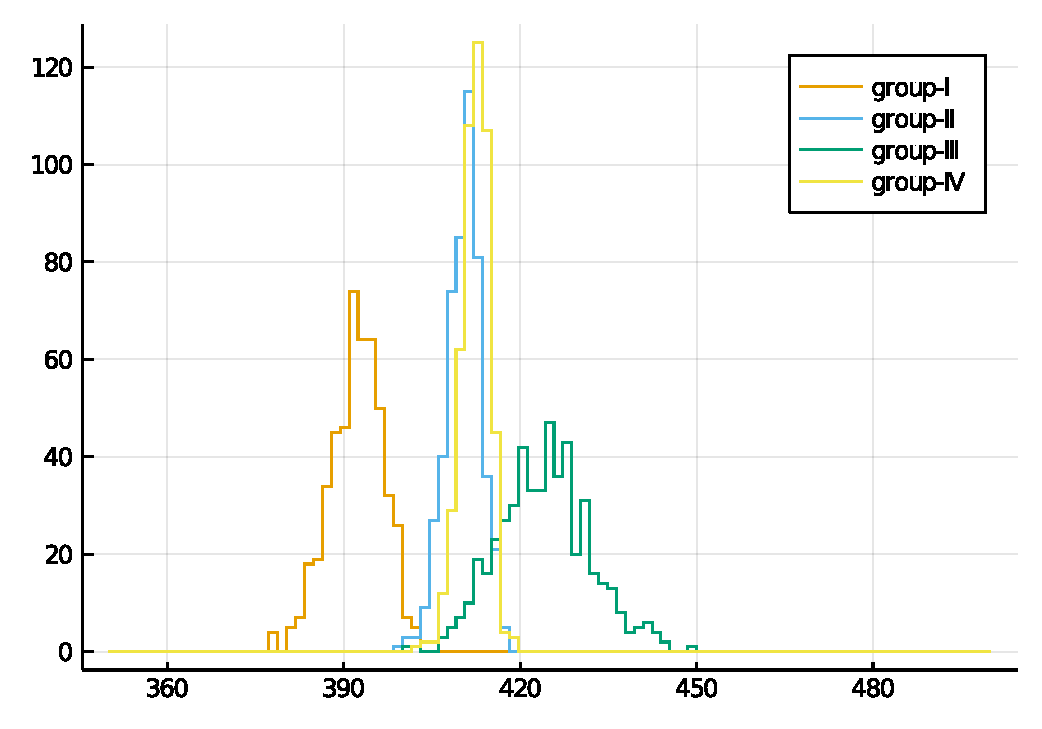
\includegraphics[width=0.48\textwidth]{../plots/llh_testing_higgs.pdf}
  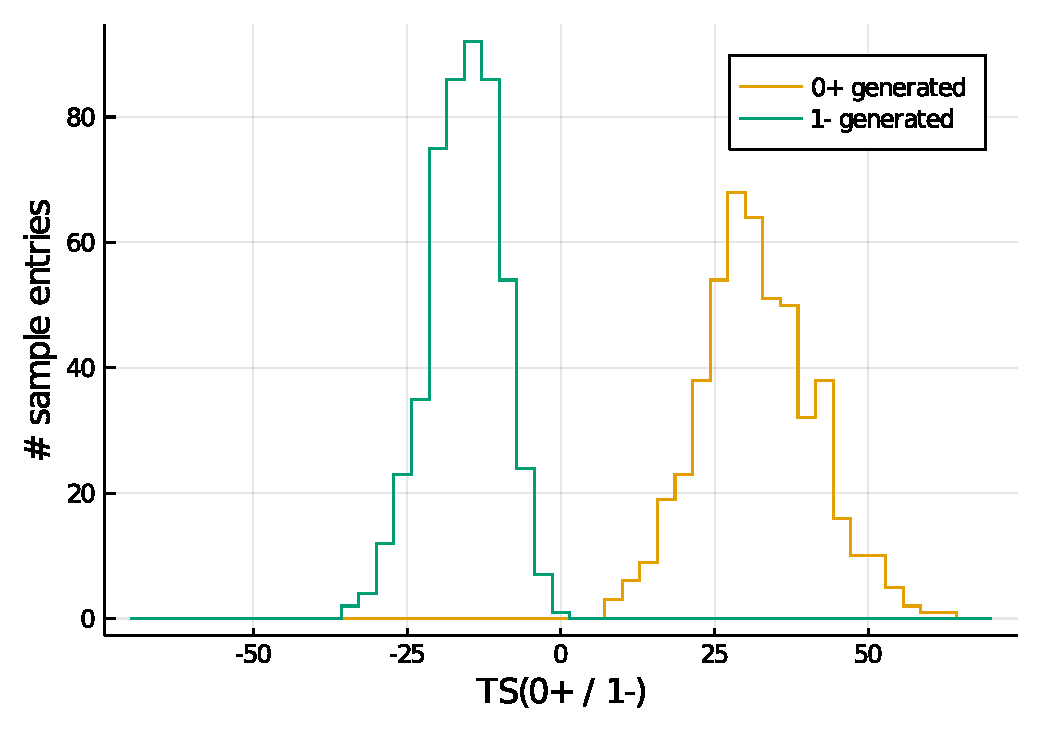
\includegraphics[width=0.48\textwidth]{../plots/TS_0p_vs_1m.pdf}
  \caption{Test statistics distribution testing hypothesis of groups $\I-\IV$ and the special cases on the statistical ensemble of the $500$ events data samples generated based on
  the fixed group-$\III$ coupling matrix. }
  \label{fig:TS.fixedH}
\end{figure}
One finds that the group-$\I$ hypothesis over-perform others in average despite statistics fluctuations.
The separation is even larger once the test statistics from Eq.~\eqref{eq:test.statistics} is computed for every sample in the poll.
The right panel of Fig.~\ref{fig:TS.fixedH} shows the comparison of the group-$\I$ and the selected alterative hypotheses, the group-$\III$.
The distribution for $\TS_{0^+/1^-}$ is entirely above zero.
The test statistics on the $1^-$ generated data is calculated by creating the second poll corresponding to the matrix $H_\III$ with $a = 1/\sqrt{3}$.
The $1^-$ hypothesis is found to have the highest likelihood in average over the second poll as also reflected by the green distribution
in right panel of Fig.~\ref{fig:TS.fixedH}. As stressed above, an important part of the separation power comes from the $\Delta\phi$ distribution.
Fig.~\ref{fig:higgs.phi} an example of $\diff N / \diff \phi$ for the two combined sample of the first poll.
\begin{figure}
  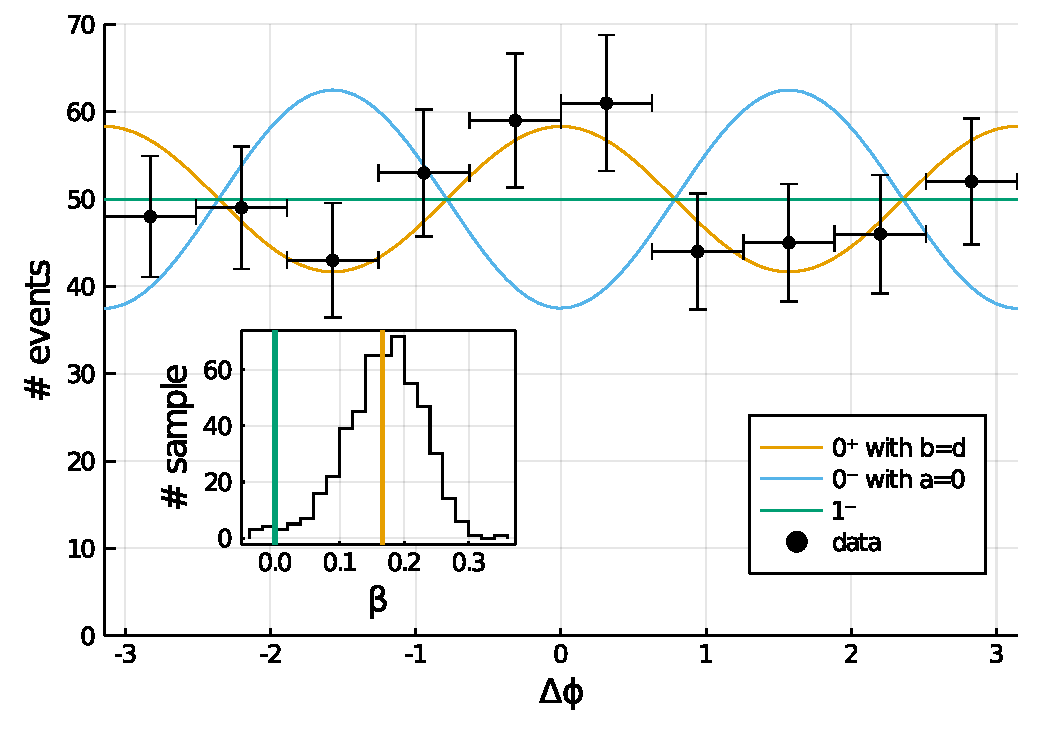
\includegraphics[width=0.48\textwidth]{../plots/phi_higgs.pdf}
  \caption{Distribution of the polar angle $\Delta\phi$ for the Higgs decay to $\mu^+\mu^-\mu^+\mu^-$ with $1000$ synthetic events.
  The orange line is the expectation curve under the $J^P=0^+$ hypotheses.
  The distribution is expected to be flat if $J$ is odd.
  The blue line gives an example of the even-unnatural $J^P$ quantum numbers (group-\II).}
  \label{fig:higgs.phi}
\end{figure}

\section{Conclusion}
We have derived an amplitude for the hadronic production of two identical vector-meson system in a model-independent framework.
As resonances lead to the structured angular distributions due to well-definite $J^P$ quantum numbers,
we show that four groups of $J^P$ separated by the parity of $J$ and the naturality of $J^P$ can be distinguish based on angular distributions.
The test-statistics discriminator is proposed.
The power of the three-dimensional analysis is demonstrated using the Standard Model Higgs decay to a pair of the $Z$ bosons.

\section*{Acknowledgement}
The project was motivated by a discussion in the LHCb Amplitude Analysis group.
We thank Biplab Day for organizing seminar dedicated to $X\to VV$.
We would like to gratefully thank Alessandro Pilloni for useful comments on the work.
We thank Liupan An and Ronan McNulty for finding practical cases for the analysis.

\appendix

\section{Modifications for $X\to V(K^+K^-)V(K^+K^-)$}

The only place that requires modification when the $\phi\phi$ system is considered
is the decay matrix element in Eq.~\eqref{eq:decay.A}:
\begin{align}
  A^{\nu}(\theta_1,\theta_2,\Delta\phi) &= 3
  \sum_{\lambda_1,\lambda_2}
  \delta_{\nu,\lambda_1-\lambda_2} (-1)^{1-\lambda_2}
  H_{\lambda_1\lambda_2}
  d_{\lambda_1,0}^{1}(\theta_1) d_{\lambda_2,0}^{1}(\theta_2)
  e^{i\lambda_2 \Delta\phi}
\end{align}
where the decay $\phi\to K^+K^-$ proceeds in $P$-wave only.

\section{Polarization vectors}

For calculation of the Higgs decay ampluitude in Eq.~\eqref{eq:HZZ}
we used explicit expressions for the polarization vectors:
\begin{align}
  \epsilon_z^{\mu}(\pm1) &= \frac{1}{\sqrt{2}} \left( 0,\mp 1,-i,0 \right), &
  \epsilon_z^{\mu}(0) &= \frac{1}{m_Z} \left(p,0,0,E\right),
\end{align}
where $E$, $p$, and $m_Z$ are the energy, momentum, and the mass of the $Z$ boson.
The general expressions for the rotational vectors follows:
\begin{align}
  % \epsilon_1(\pm1) &= R_z(\Delta\phi) R_y(\theta) (0,-i,\mp 1,0)\frac{1}{\sqrt{2}},\\
  % \epsilon_2(\pm1) &= R_z(\Delta\phi) R_y(\theta) R_y(\pi) (0,-i,\mp 1,0)\frac{1}{\sqrt{2}};\\
  % \epsilon_1(0) &= R_z(\Delta\phi) R_y(\theta) (-p,0,0,E)\frac{1}{m},\\
  % \epsilon_2(0) &= (-1) R_z(\Delta\phi) R_y(\theta) R_y(\pi) (-p,0,0,E)\frac{1}{m},
  \epsilon_1(\lambda) &= R_z(\phi) R_y(\theta) \epsilon_z(\lambda),\\
  \epsilon_2(\lambda) &= (-1)^{1-\lambda} R_z(\phi) R_y(\theta) R_y(\pi) \epsilon_z(\lambda),\\
\end{align}
where $R_y(\phi)R_y(\theta)$ is a product of the three-dimensional rotation matrices
that transforms the vector $(0,0,1)$ to the direction $(\sin\theta\cos\phi,\,\sin\theta\sin\phi,\,\cos\theta)$.
The particle-2 requires additional rotation by $\pi$ about the $y$ axis. We also use the particle-two phase convention,
$(-1)^{1-\lambda_2}$ that adds an extra sign to the vector $\epsilon_2(0)$.

\section{$\eta s$ invariance}
The helicity coupling matrices in Eq.~\eqref{eq:matrices} are all orthogonal to each other,
with the scaler product given by $(H_1\cdot H_2) = \mathrm{Tr}(H_1 H_2^\dagger)$.
Nevertheless, there are potential cases where different hypothesis are not distinguishable.
An example that demonstrate such degeneracy is the following:
\begin{equation}
  H^{(\text{deg.})} = \begin{pmatrix}
    0 &1 &0 \\
    s & 0 &s\eta \\
    0 &\eta &0
  \end{pmatrix},
\end{equation}
where $s$ is the parity of $J$, and $\eta$ is the naturality of $J^P$.
The matrix of this type is present in all groups for different values of $s$ and $\eta$

The intensity of the unpolarized decay can be computed explicitly~\cite{7717/peerj-cs.103}:
\begin{align}
  I(H) &= \frac{s^{2} \eta^{2} \sin^{2}{\left (\theta_{1} \right )} \cos^{2}{\left (\theta_{2} \right )}}{2} + \frac{s^{2} \eta^{2} \sin^{2}{\left (\theta_{1} \right )}}{2} + \frac{s^{2} \sin^{2}{\left (\theta_{1} \right )} \cos^{2}{\left (\theta_{2} \right )}}{2} + \frac{s^{2} \sin^{2}{\left (\theta_{1} \right )}}{2} \\ \nonumber
   &\quad + \frac{s \eta \left(\cos{\left (- 2 \theta_{1} + 2 \theta_{2} + \Delta\phi \right )} + \cos{\left (2 \theta_{1} - 2 \theta_{2} + \Delta\phi \right )} - \cos{\left (2 \theta_{1} + 2 \theta_{2} - \Delta\phi \right )} - \cos{\left (2 \theta_{1} + 2 \theta_{2} + \Delta\phi \right )}\right)}{8}\\ \nonumber
   &\quad+\frac{\eta^{2} \sin^{2}{\left (\theta_{2} \right )} \cos^{2}{\left (\theta_{1} \right )}}{2} + \frac{\eta^{2} \sin^{2}{\left (\theta_{2} \right )}}{2} + \frac{\sin^{2}{\left (\theta_{2} \right )} \cos^{2}{\left (\theta_{1} \right )}}{2} + \frac{\sin^{2}{\left (\theta_{2} \right )}}{2}
\end{align}
The expression does not change under the flip of $\eta$ and $s$ sign simultaneously.
Hence, the group-$\II$ with $и=0$ is undistinguished from the group-$\III$,
and the group-$\I$ with $b=d=c=0$ have the same angular distributions as the group-$\IV$ with $c=0$.
Such vanishing of the helicity couplings, however, must be an exceptional case indicating some peculiar physical reason.

\bibliography{ref}
\end{document}




% \begin{align}
%   \frac{\diff^2 N}{\diff \cos\theta_1\,\diff \cos\theta_2} =
%   |H_{\lambda_1\lambda_2}|^2
%   \sum_{\xi_1,\xi_2}^{\{-1,1\}}
%   9|d_{\lambda_1,\xi_1}^{1}(\theta_1) d_{\lambda_2,\xi_2}^{1}(\theta_2)|^2.
% \end{align}

% \section{LS couplings}
%
% \begin{align}
%   H_{\lambda_1,\lambda_2} = (-1)^{j_2-\lambda_2} \sum_{ls} \sqrt{\frac{2l+1}{2j+1}}
%   \left\langle 1,\lambda_1;1,\lambda_2|s,\lambda_1-\lambda_2 \right\rangle
%   \left\langle L,0;s,\lambda_1-\lambda_2|j,\lambda_1-\lambda_2 \right\rangle H_{ls}.
% \end{align}
%
% \begin{align*}
%   1^-\otimes 1^-: && S:\qquad & {\color{cola} 0^+}\quad {\color{colb} 1^+}\quad {\color{colc} 2^+},\\
%                   && P:\qquad & \color{gray} 1^-\quad (0^-,1^-,2^-)\quad (1^-,2^-,3^-),\\
%                   && D:\qquad & {\color{colc} 2^+}\quad ({\color{colb} 1^+},{\color{colc} 2^+},3^+)\quad ({\color{cola} 0^+},{\color{colb} 1^+},{\color{colc} 2^+},3^+,4^+),\\
%                   && F:\qquad & \color{gray} 3^-\quad (2^-,3^-,4^-)\quad (0^-,1^-,2^-,3^-,4^-),\\
%                   && H:\qquad & 4^+\quad (3^+,4^+,5^+)\quad ({\color{colc} 2^+},3^+,4^+,5^+,6^+).
% \end{align*}

% \section{Odd and even spins}

% \begin{figure}
%   \includegraphics[width=0.46\textwidth]{../plots/moment_M2phi_Nev=500.pdf}
%   \caption{Distribution of $M_{\cos(2\Delta\phi)}$ for a sample of random coupling constants.
%   A sample of $500$ events is generated for every hypothesis of couplings.}
%   \label{}
% \end{figure}
%
% \begin{figure}
%   \includegraphics[width=0.9\textwidth]{../plots/llh_of_fit_of_J012.pdf}
%   \caption{Hypothesis testing with $500$ events}
%   \label{fig.3dfit}
% \end{figure}


% Matrices of couplings without the phase $(-1)^{j_2-\lambda_2}$ are symmetric (round brackets) or asymmetric (square parentheses)
% \begin{itemize}
%   \item $j = 0$:
% \begin{align*}
%   % l = 0, s = 0
%   \frac{\sqrt{3}}{3}
%   \begin{pmatrix}1 & 0 & 0\\0 & -1 & 0\\0 & 0 & 1\end{pmatrix}&&
%   % l = 2, s = 2
%   \frac{\sqrt{6}}{6}
%   \begin{pmatrix}1 & 0 & 0\\0 & 2 & 0\\0 & 0 & 1\end{pmatrix}
% \end{align*}
%   \item $j = 1$:
% \begin{align*}
%   % l = 0, s = 1
%   \frac{\sqrt{6}}{6}
%   \begin{pmatrix}-1 & -1 & 0\\-1 & 0 & 1\\0 & 1 & 1\end{pmatrix}&&
%   % l = 2, s = 1
%   \frac{\sqrt{3}}{6}
%   \begin{pmatrix}2 & -1 & 0\\-1 & 0 & 1\\0 & 1 & -2\end{pmatrix}&&
%   % l = 2, s = 2
%   \frac{1}{2}
%   \left[\begin{matrix}0 & -1 & 0\\1 & 0 & -1\\0 & 1 & 0\end{matrix}\right]
% \end{align*}
% \item $j = 2$:
% \begin{align*}
%   % l = 0, s = 2
%   \frac{\sqrt{30}}{30}
%   \begin{pmatrix}1 & \sqrt{3} & \sqrt{6}\\\sqrt{3} & 2 & \sqrt{3}\\\sqrt{6} & \sqrt{3} & 1\end{pmatrix}&&
%   % l = 2, s = 0
%   \frac{\sqrt{3}}{3}
%   \begin{pmatrix}1 & 0 & 0\\0 & -1 & 0\\0 & 0 & 1\end{pmatrix}&&
%   % l = 2, s = 1
%   \frac{1}{2}
%   \left[\begin{matrix}0 & -1 & 0\\1 & 0 & 1\\0 & -1 & 0\end{matrix}\right]&&
%   % l = 2, s = 2
%   \frac{\sqrt{7}}{14}
%   \begin{pmatrix}- \frac{2 \sqrt{3}}{3} & -1 & 2 \sqrt{2}\\-1 & -\frac{4 \sqrt{3}}{3} & -1\\2 \sqrt{2} & -1 & - \frac{2 \sqrt{3}}{3}\end{pmatrix}&&
%   % l = 4, s = 2
%   \frac{\sqrt{70}}{70}
%   \begin{pmatrix}\sqrt{6} & -2 \sqrt{2} & 1\\- 2 \sqrt{2} & 2\sqrt{6} & - 2 \sqrt{2}\\1 & -2\sqrt{2} & \sqrt{6}\end{pmatrix}
% \end{align*}
% \end{itemize}
%
% \begin{figure}
%   \includegraphics[width=0.195\textwidth]{../plots/map_JLS_000.pdf}
%   \includegraphics[width=0.195\textwidth]{../plots/map_JLS_022.pdf}
%   \caption{}
%   \label{fig.j0}
% \end{figure}
% \begin{figure}
%   \includegraphics[width=0.195\textwidth]{../plots/map_JLS_101.pdf}
%   \includegraphics[width=0.195\textwidth]{../plots/map_JLS_121.pdf}
%   \includegraphics[width=0.195\textwidth]{../plots/map_JLS_122.pdf}
%   \caption{}
%   \label{fig.j1}
% \end{figure}
% \begin{figure}
%   \includegraphics[width=0.195\textwidth]{../plots/map_JLS_202.pdf}
%   \includegraphics[width=0.195\textwidth]{../plots/map_JLS_220.pdf}
%   \includegraphics[width=0.195\textwidth]{../plots/map_JLS_221.pdf}
%   \includegraphics[width=0.195\textwidth]{../plots/map_JLS_222.pdf}
%   \includegraphics[width=0.195\textwidth]{../plots/map_JLS_242.pdf}
%   \caption{}
%   \label{fig.j2}
% \end{figure}


% \begin{align}
%     I(\cos\theta_1,\phi_1,\cos\theta_2,\phi_2) &= 9\sum_{M}P_M
%     \sum_{\lambda_1,\lambda_2}\sum_{\lambda_1',\lambda_2'}
%     d_{M,\lambda_1-\lambda_2}^{J}(\theta) (-1)^{1-\lambda_2}
%     d_{M,\lambda_1'-\lambda_2'}^{J}(\theta) (-1)^{1-\lambda_2'}
%     \\ \nonumber
%     &\qquad\times
%     H_{\lambda_1\lambda_2} H_{\lambda_1'\lambda_2'}^{*}
%     e^{i(\lambda_1'-\lambda_1)\phi_1}
%     e^{i(\lambda_2'-\lambda_2)\phi_2}
%     \\ \nonumber
%     &\qquad\times
%     \sum_{\xi_1}^{\{-1,1\}}
%     d_{\lambda_1,\xi_1}^{1}(\theta_1) d_{\lambda_1',\xi_1}^{1}(\theta_1)
%     \sum_{\xi_2}^{\{-1,1\}}
%     d_{\lambda_2,\xi_2}^{1}(\theta_2) d_{\lambda_2',\xi_2}^{1}(\theta_2).
% \end{align}
